\section{Results}

\subsection{Sensitivity analysis}

\begin{figure}
  \centering
  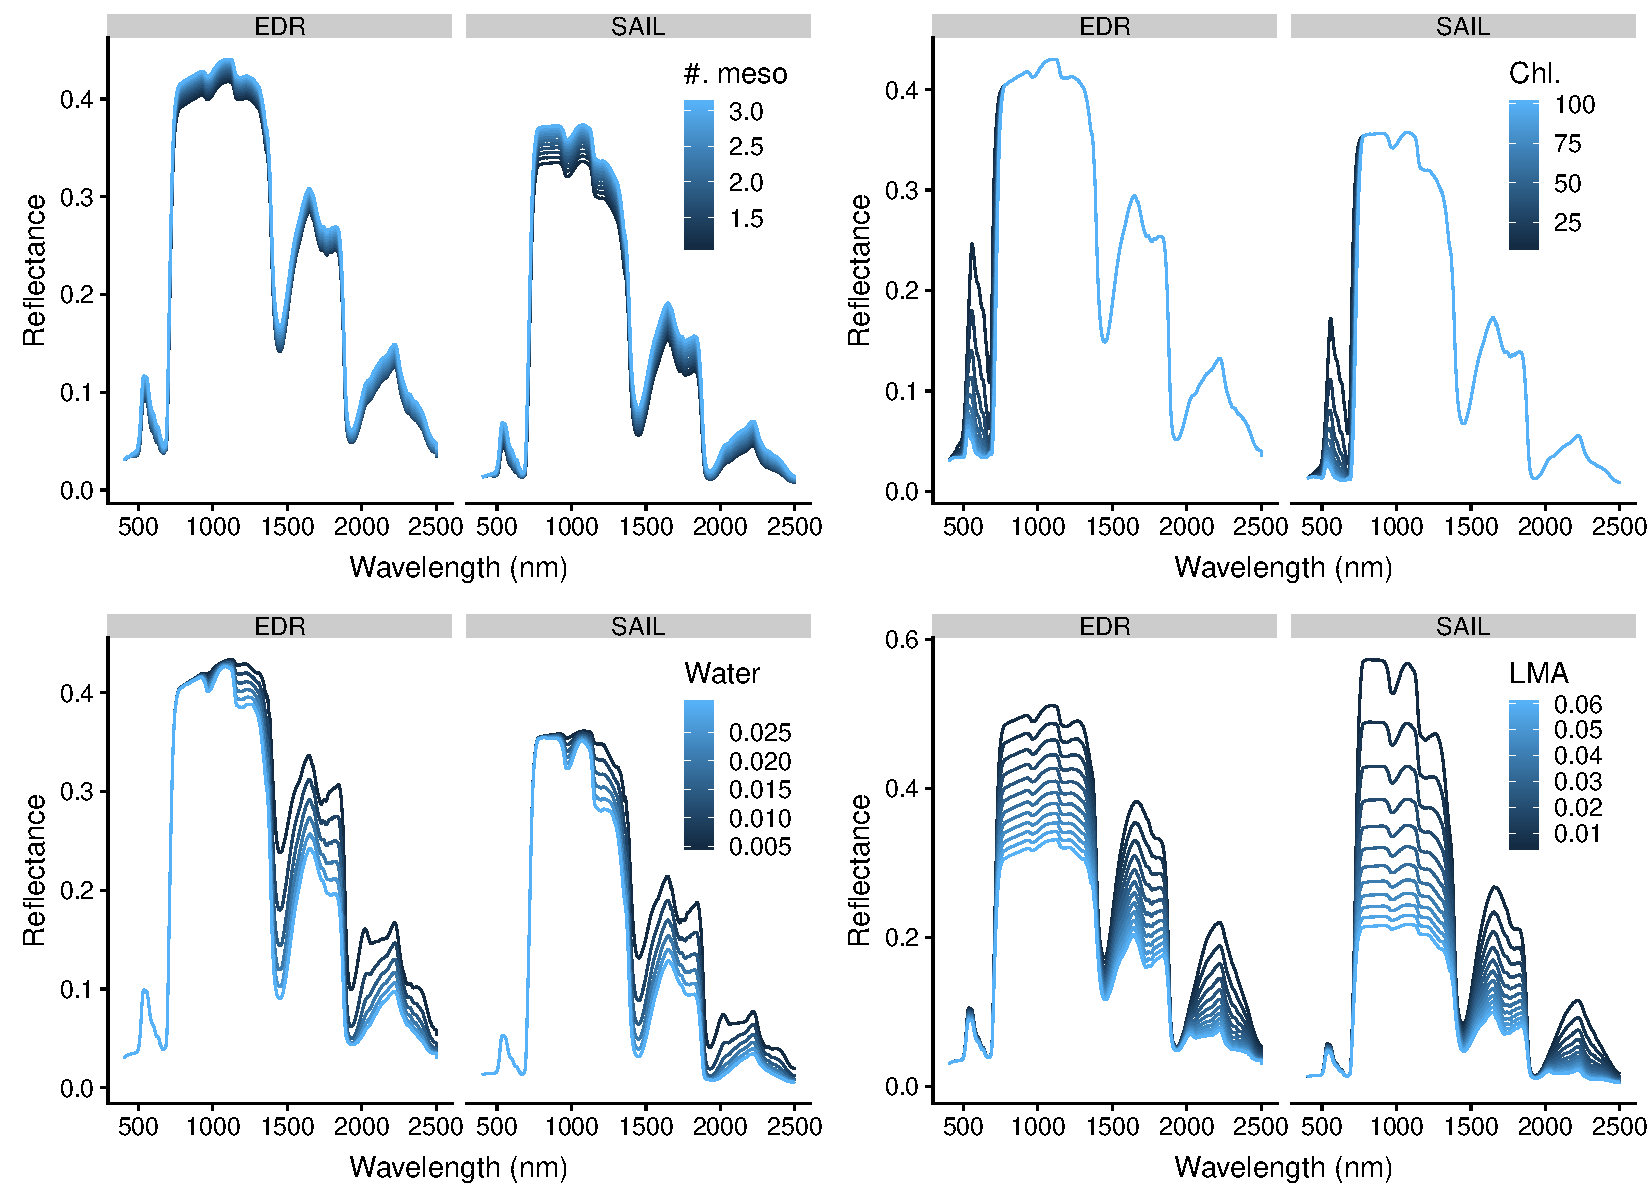
\includegraphics[width=\textwidth]{4_edr/figures/explore_spectra/edr_sensitivity_leaf_single.pdf}
  \caption{\
    Sensitivity of EDR and 4SAIL predicted canopy reflectance to leaf optical traits.
    For all figures, leaf area index is fixed at 4.88.
    EDR simulations are for a single-cohort canopy (Early Hardwood) with
    clumping factor 0.09 and orientation factor 0.06.
    4SAIL predictions are for directional-hemispherical reflectance.
  }\label{fig:sensitivity_leaf_single}
\end{figure}

The general character of the sensitivities of EDR and 4SAIL to leaf optical properties is similar,
but the magnitudes of these sensitivites are different (Figure~\ref{fig:sensitivity_leaf_single}).
EDR consistently shows significantly higher reflectance across most of the spectrum than 4SAIL\@.
Sensitivity to leaf mesophyll structure is lower in EDR than 4SAIL, while sensitivity for chlorophyll and water contents is comparable.
Sensitivity to leaf dry mass per area is comparable for both models in the shortwave infrared, but significantly higher for 4SAIL in the near infrared.

\begin{figure}
  \centering
  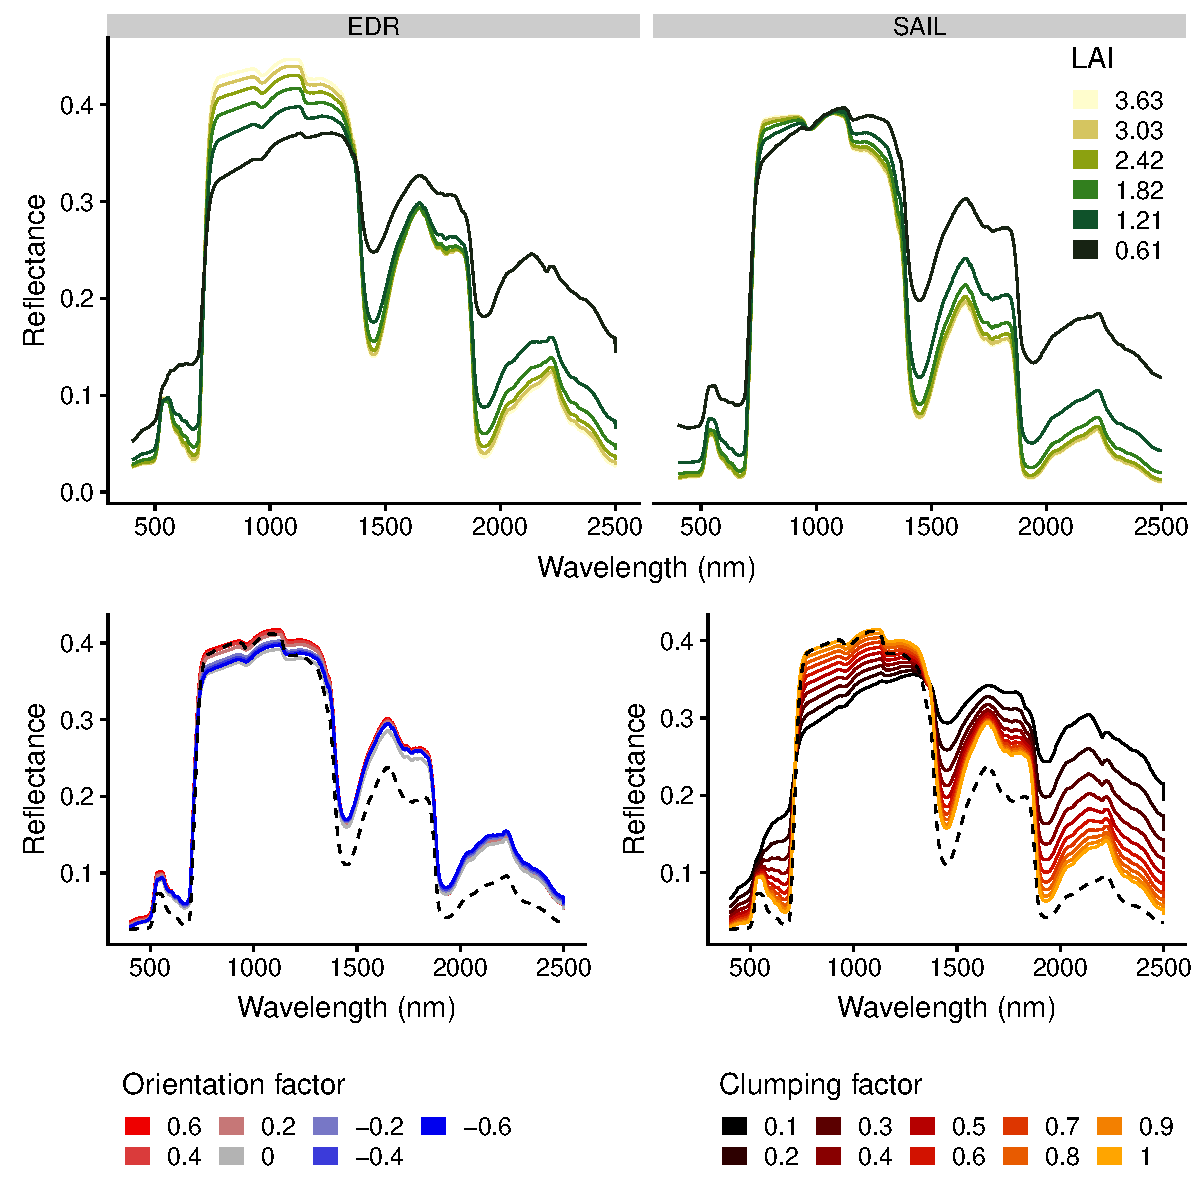
\includegraphics[width=\textwidth]{4_edr/figures/explore_spectra/sensitivity_single_pft.pdf}
  \caption{\
    Sensitivity of EDR and 4SAIL predicted canopy reflectance to leaf area index (\textit{top}) and leaf orientation factor (\textit{middle}).
    (\textit{Bottom}) Sensitivity of EDR predicted canopy reflectance and clumping factor,
    with dashed line indicating 4SAIL predictions for the same leaf area index, PROSPECT parameters, and approximately equivalent soil background.
    Configuration is the same as in Figure~\ref{fig:sensitivity_leaf_single}.
  }\label{fig:sensitivity_structure_single}
\end{figure}

EDR and 4SAIL show different responses to leaf area index (Figure~\ref{fig:sensitivity_structure_single}).
Although both models predict declines in reflectance with increasing leaf area in the visible and shortwave infrared range,
4SAIL also predicts a decline in the near infrared while EDR predicts an increase.
The sensitivities of both models to leaf area index are also different.
4SAIL predicts more reflectance sensitivity at low leaf area indices and saturation of reflectance around 4, while EDR shows a more gradual decline in sensitivity, particularly in the near-infrared range. 
An important caveat to these results is that, particularly at low leaf area index, they are strongly dependent on the value of the background soil reflectance.
To match the EDR default (see Methods), 4SAIL was configured with a relatively bright soil reflectance (i.e.\ a fairly dry soil), which explains the decline in near-infrared reflectance as leaf area increases.
When the soil background is dark, SAIL shows increasing near-infrared reflectance with increasing leaf area (but saturating to the same value as the contribution of the soil background becomes negligible at high leaf area).

Similarly to leaf area, EDR and 4SAIL agree on the directionality leaf orientation effects on reflectance (declining reflectance with increasingly vertical leaves), but differ in their sensitivities, with EDR having a much lower sensitivity to changing leaf angles.
Finally, sensitivity of EDR to canopy clumping is nearly identical to that of leaf area index, which makes sense given the interaction between these terms in defining canopy transmissivity (Equations~\ref{eq:tau_r} and~\ref{eq:tai}).

\begin{figure}
  \centering
  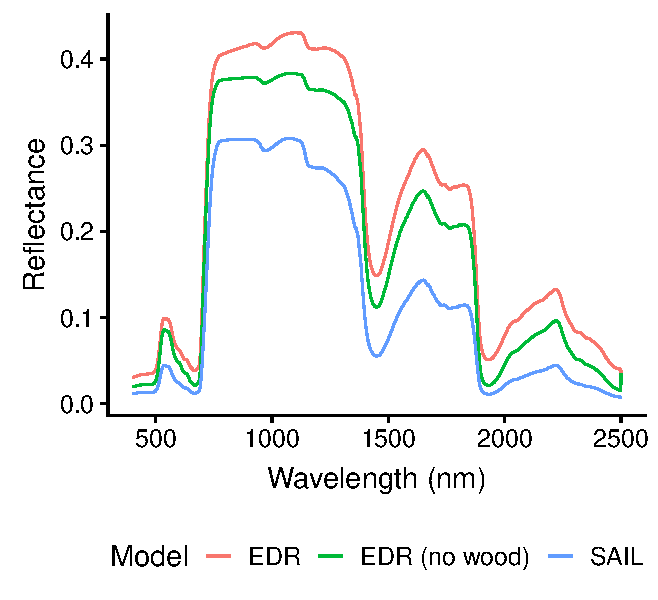
\includegraphics{4_edr/figures/explore_spectra/edr_wood_compare.pdf}
  \caption{\
    Comparison of predicted canopy reflectance by 4SAIL (directional-hemispherical) and EDR with and without wood reflectance included.
  }\label{fig:wood_compare}
\end{figure}

Compared to 4SAIL, EDR consistently overpredicts canopy reflectance across the entire spectrum (Figures~\ref{fig:sensitivity_leaf_single},~\ref{fig:sensitivity_structure_single}, and~\ref{fig:wood_compare}).
A significant part of this bias can be explained by the inclusion of wood reflectance in EDR, but a persistent positive bias remains across most of the spectrum even after setting wood reflectance to zero (Figure~\ref{fig:wood_compare}).

\begin{figure}
  \centering
  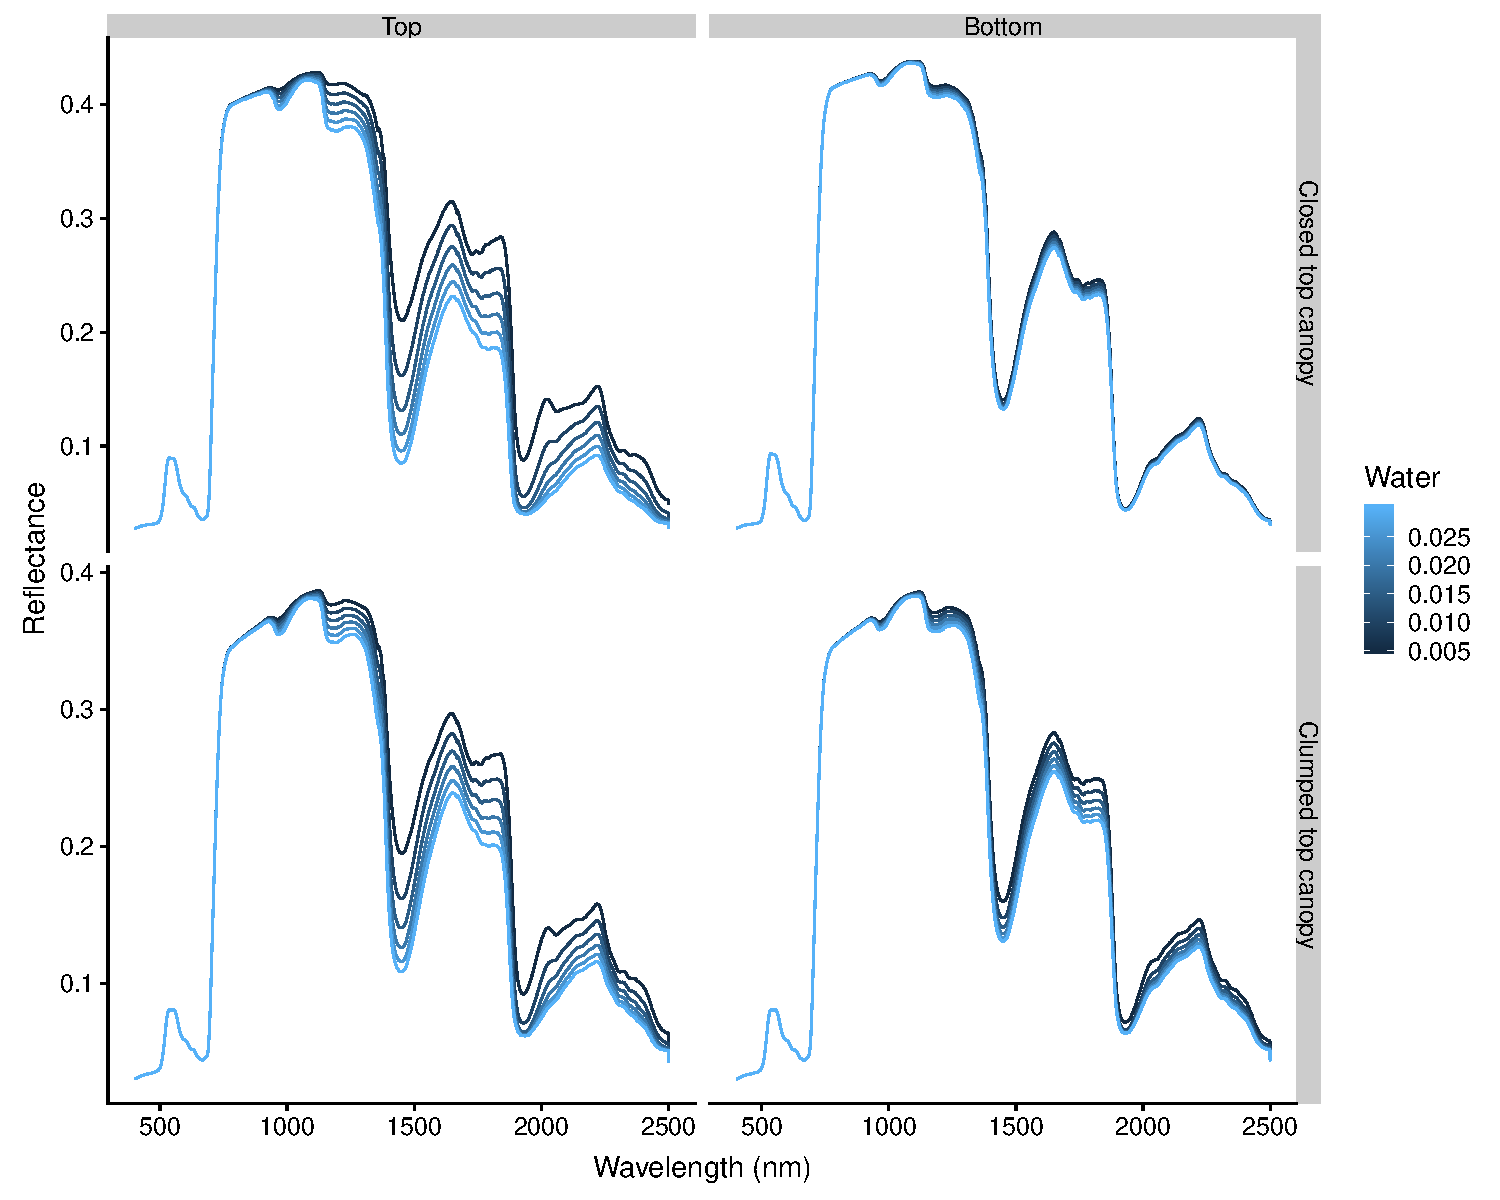
\includegraphics[width=\textwidth]{4_edr/figures/explore_spectra/edr_sensitivity_double.pdf}
  \caption{\
    Sensitivity of EDR canopy reflectance to leaf water content of top (\textit{left}) and bottom (\textit{right}) cohorts within a multi-cohort canopy,
    when the top canopy is closed (\textit{top}) and highly clumped (\textit{bottom}).
    Top and bottom cohorts are, respectively, Early and North Mid Hardwood with DBH 40 and 30, LAI 2.4 and 1.3, and equal stem density.
    Clumping factors for closed and clumped canopies are 0.9 and 0.3, respectively.
  }\label{fig:sensitivity_water_multi}
\end{figure}

EDR canopy reflectance is highly sensitive to the properties of the tallest cohort, and shows virtually no sensitivity to the optical properties of lower cohorts (Figure~\ref{fig:sensitivity_water_multi}).
Clumping (or reduced LAI) allow more light to penetrate the canopy and therefore increases the sensitivity of canopy reflectance to the properties of lower layers, but this sensitivity is effect is still significantly muted compared to the top canopy.


\subsection{Model calibration}

\begin{figure}
  \centering
  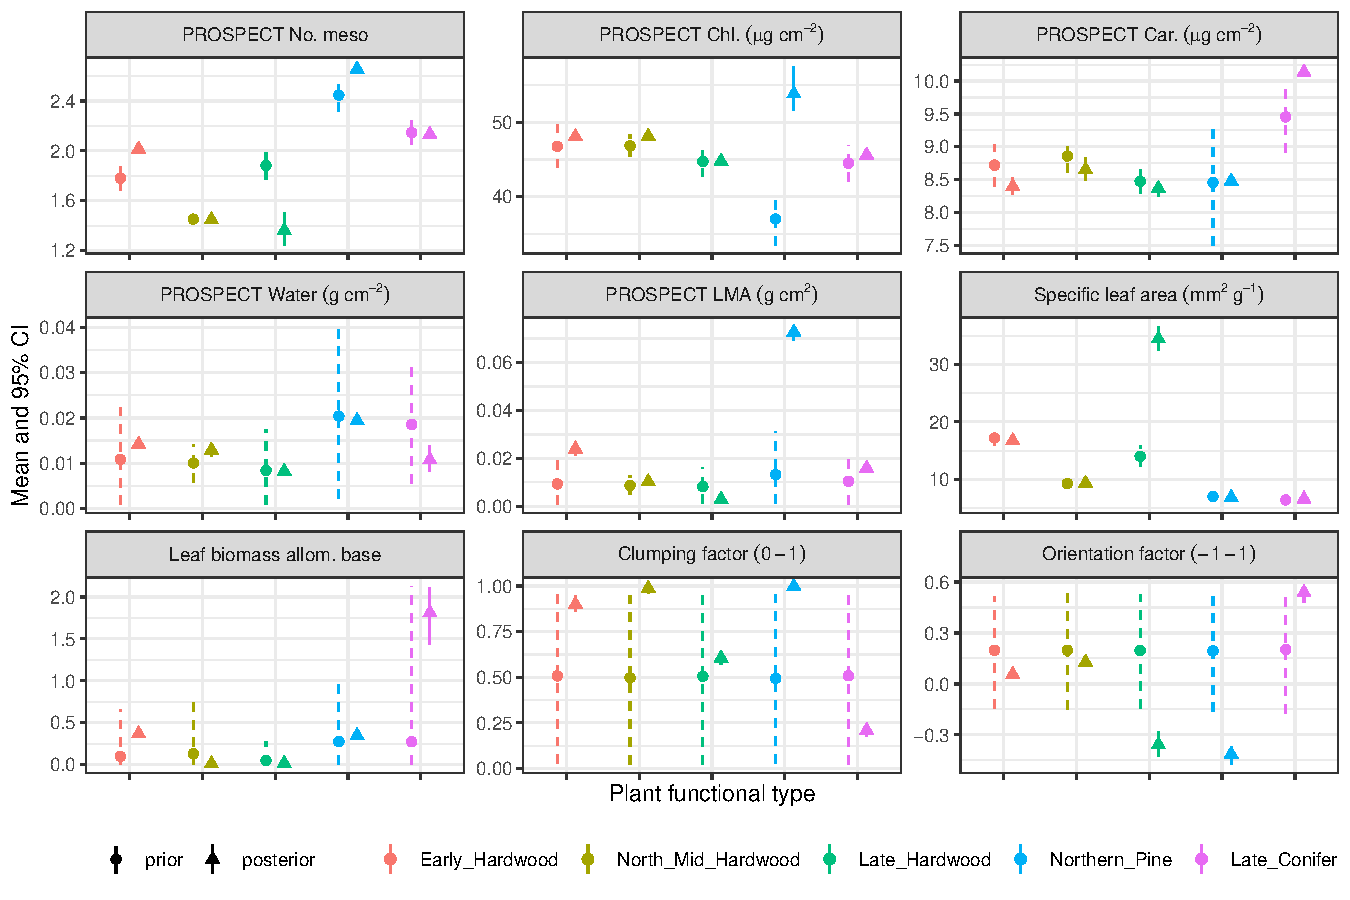
\includegraphics[width=\textwidth]{4_edr/figures/explore_spectra/pda_summary.pdf}
  \caption{\
    Summary statistics for model calibration parameter prior and posterior distributions.
  }\label{fig:pda_posteriors}
\end{figure}

Model calibration substantially improved the precision of almost all parameter estimates, even when prior distributions were strongly informative (Figure~\ref{fig:pda_posteriors}).
In most cases, the posterior distribution fell within the prior, but there were a few notable exceptions.
Specifically, northern pines had significantly higher calibration estimates of chlorophyll content and leaf mass per area and significantly lower estimates of the orientation factor (though the prior on the latter was not based on data).
Late hardwoods also had orientation factor estimates much lower than the prior, and also had significantly lower estimates of leaf mesophyll structure.

\begin{figure}
  \centering
  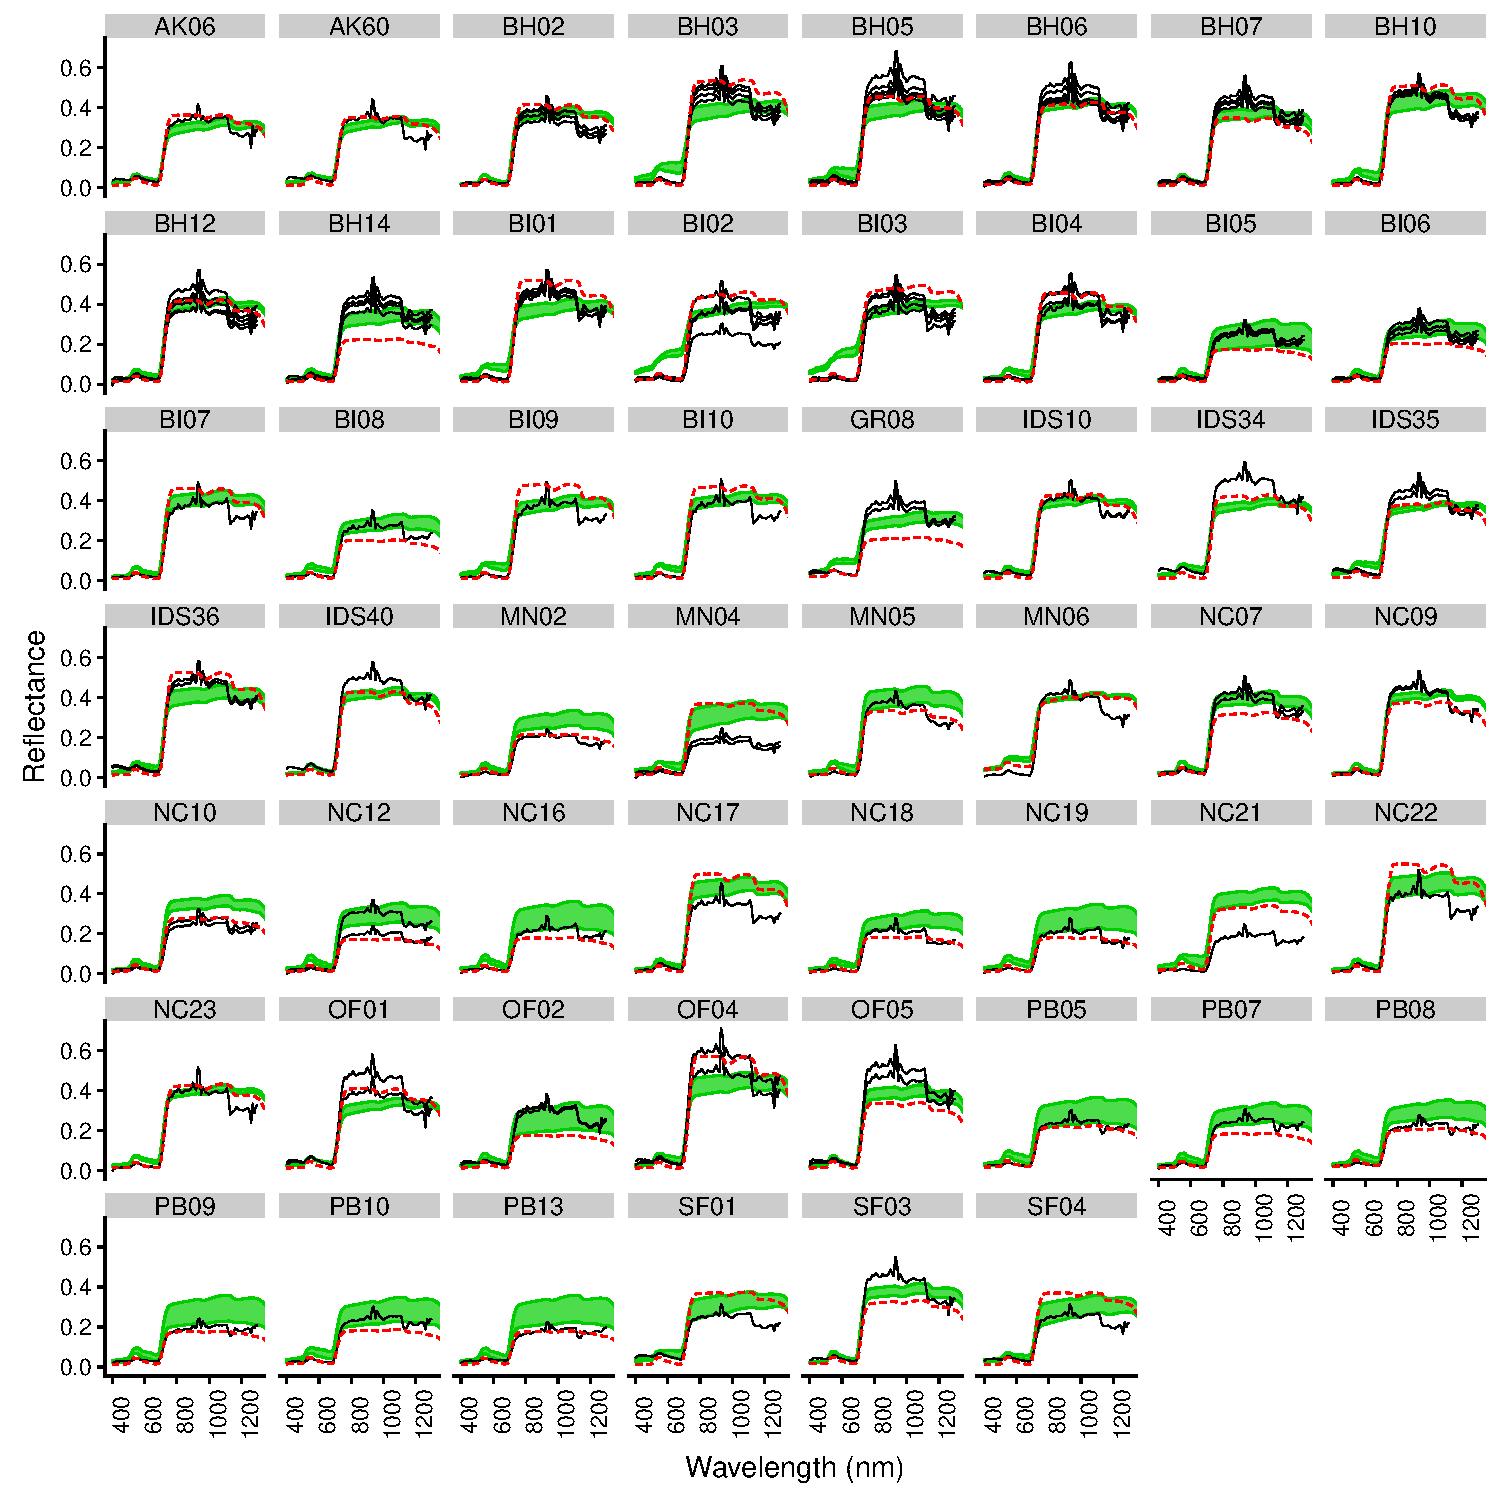
\includegraphics[width=\textwidth]{4_edr/figures/explore_spectra/errors_all.pdf}
  \caption{%
    Comparison between AVIRIS observations (black), posterior credible intervals on EDR predicted spectra (green), and posterior mean predictions using 4SAIL (red, dashed) for each site used in the calibration.
  }\label{fig:spec_error_all}
\end{figure}

\begin{figure}
  \centering
  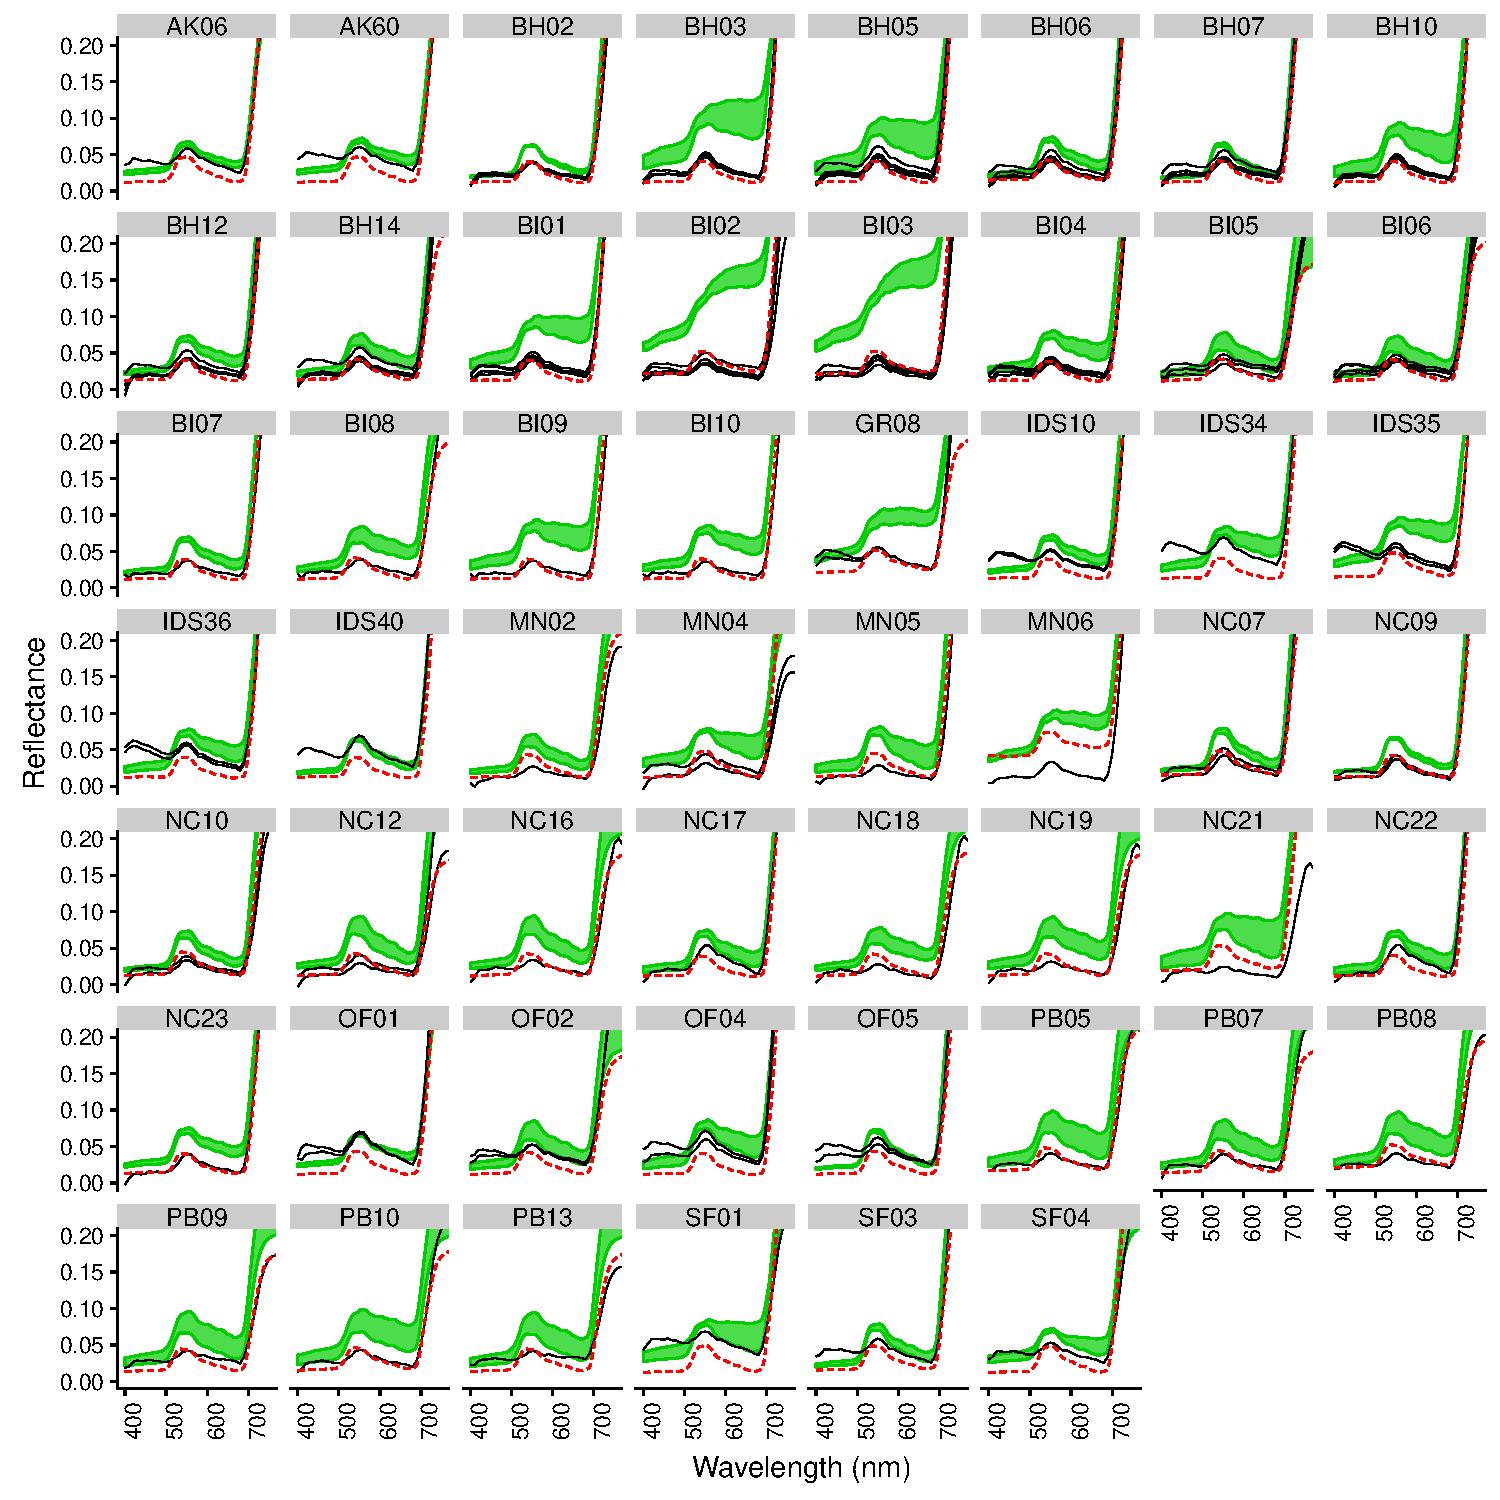
\includegraphics[width=\textwidth]{4_edr/figures/explore_spectra/errors_vis.pdf}
  \caption{%
    Same as Figure~\ref{fig:spec_error_all}, but zoomed into the visible ($<$750 nm) spectral region.
  }\label{fig:spec_error_vis}
\end{figure}

The ability of EDR to reproduce observed spectra at every site was strongly site-dependent (Figure~\ref{fig:spec_error_all}).
At a majority of the sites, EDR systematically over-predicted reflectance in the visible range (Figure~\ref{fig:spec_error_vis}), while errors in the near-infrared region were more variable.
As shown in the sensitivity analysis, this consistent over-prediction of visible reflectance is likely driven by wood reflectance (Figure~\ref{fig:wood_compare}).
4SAIL also showed a lot of site-to-site variability in its performance, but generally performed better in the visible range than EDR\@.

\begin{figure}
  \centering
  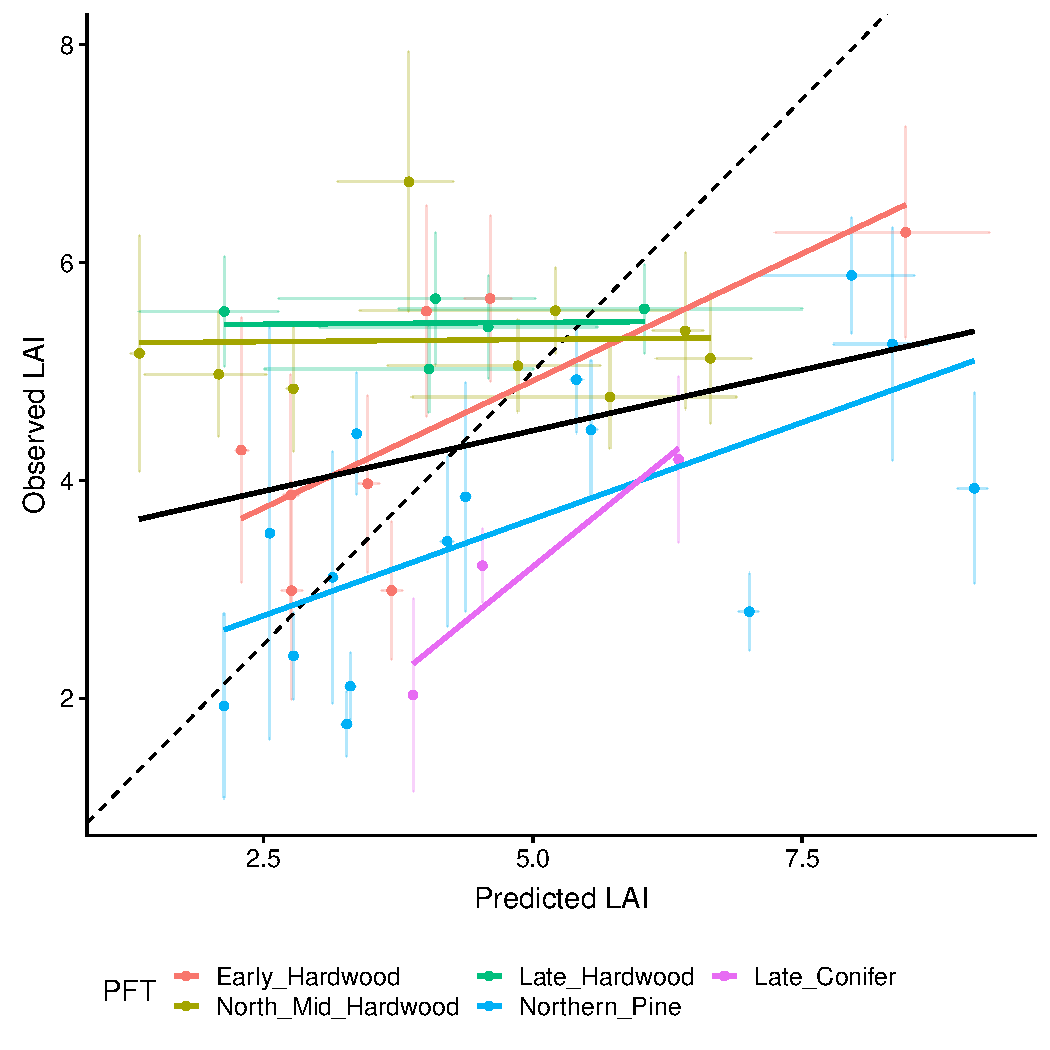
\includegraphics[width=\textwidth]{4_edr/figures/explore_spectra/lai_scatter.pdf}
  \caption{\
    Predictions of leaf area index by EDR, compared to observed values.
    Colors indicate the plant functional type of the tallest cohort at each site.
    % TODO: Add by-PFT regression line
  }\label{fig:lai_validation}
\end{figure}

The ability of EDR to reproduce observed leaf area index was also strongly site-dependent, with some of the accuracy explained by the functional type of the tallest cohort (Figure~\ref{fig:lai_validation}).
In general, EDR tended to over-predict leaf area index for conifer-dominated stands and under-predict for hardwood-dominated stands.
For mid- and late-hardwood-dominated stands in particular, EDR predicted substantial variability in leaf area index that was not present in the observations.

\begin{figure}
  \centering
  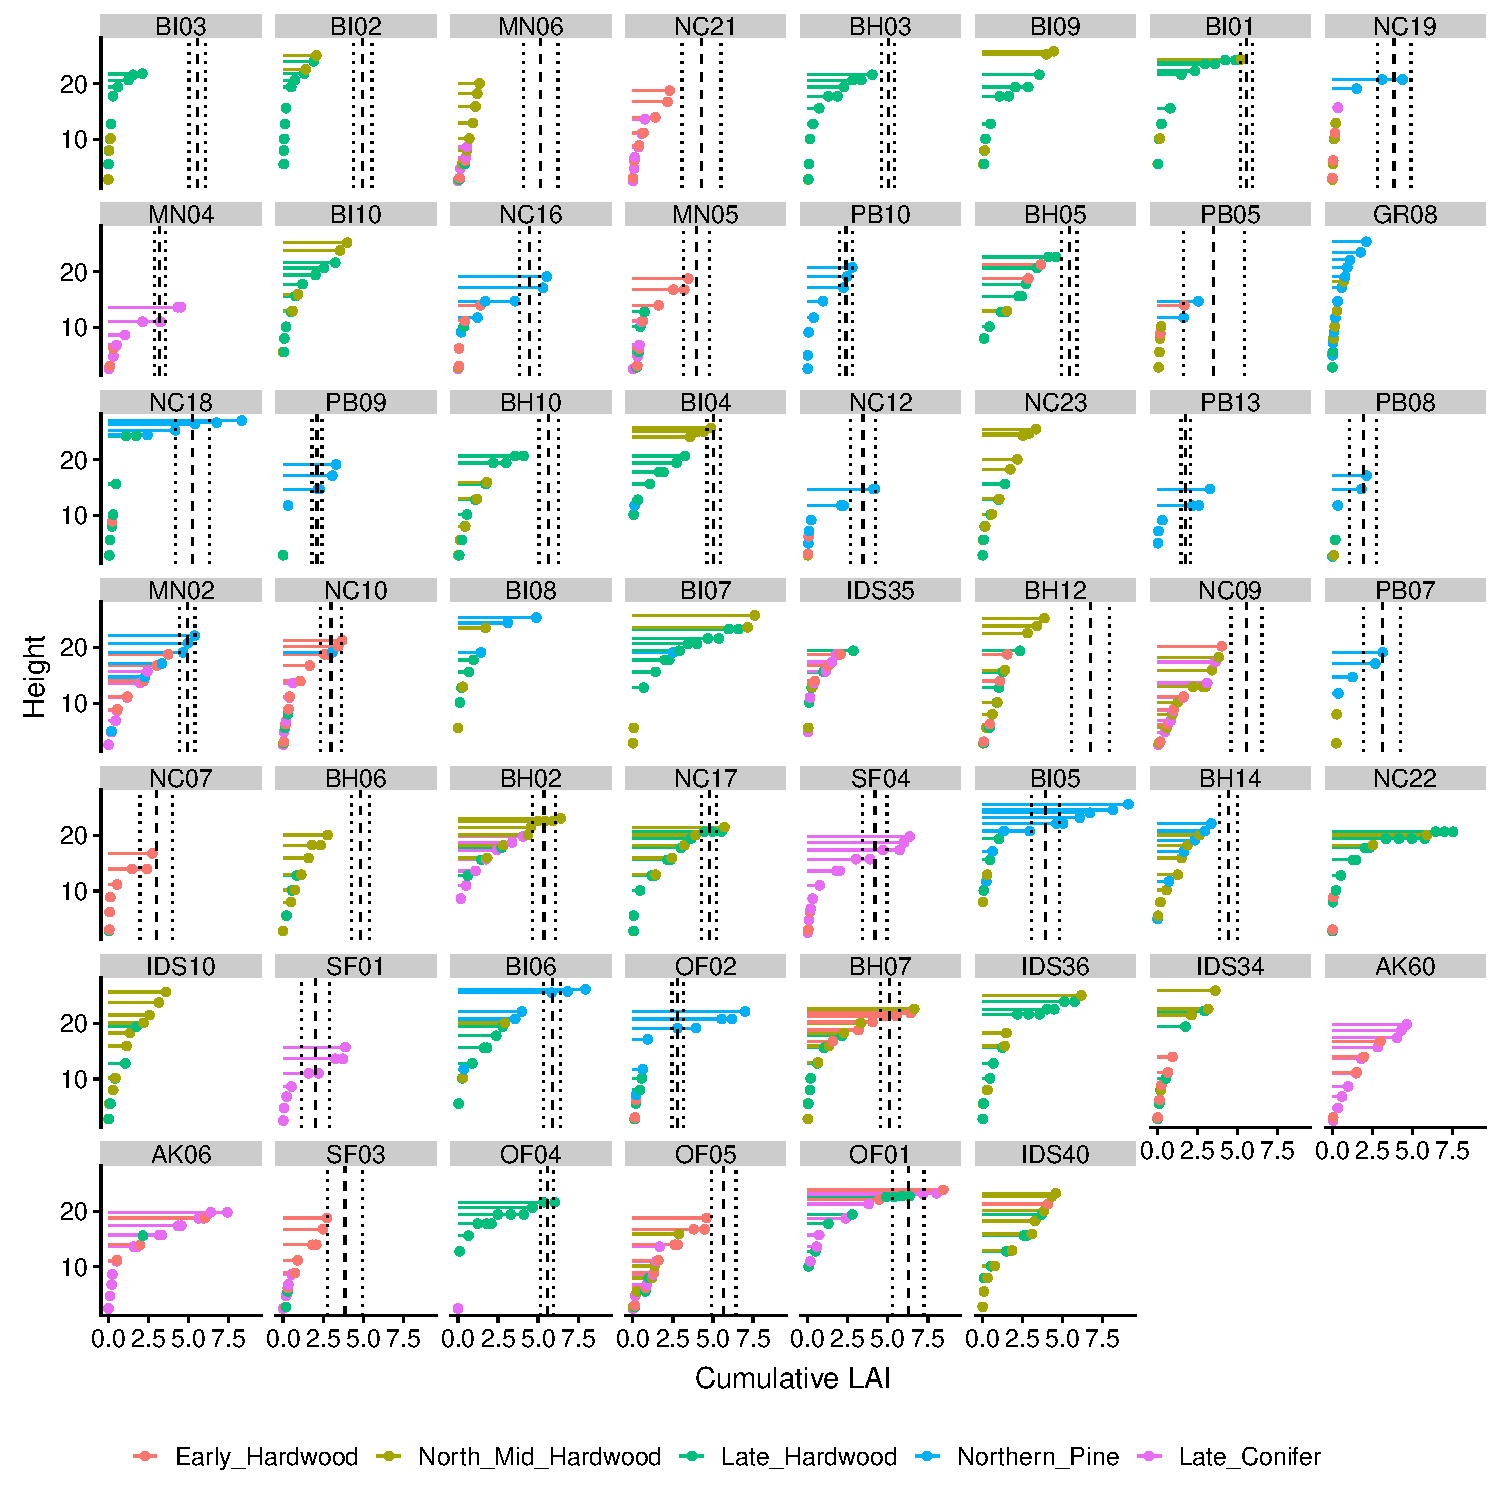
\includegraphics[width=\textwidth]{4_edr/figures/explore_spectra/ed_cumlai_plot.pdf}
  \caption{%
    Vertical profile of cumulative leaf area index and composition at each site in this analysis.
    Vertical black lines indicate the mean $\pm$ 1 standard deviation of the observed leaf area index.
    Sites are arranged in the same order as Figures~\ref{fig:spec_error_all} and~\ref{fig:spec_error_vis}.
  }\label{fig:lai_profile}
\end{figure}

Mismatch between EDR predictions and AVIRIS reflectance were likely caused by a number of factors related to site composition and structure (Figures~\ref{fig:spec_error_vis} and~\ref{fig:lai_profile}).
In some sites, the mismatch was most likely due to a mismatch in leaf area index, such as BI02, BI03, and MN06.
Notably, at BI02 and BI03 (and several other sites), EDR and 4SAIL show opposite biases---EDR over-predicts visible reflectance but successfully captures the near-infrared reflectance, while 4SAIL does the opposite (Figure~\ref{fig:spec_error_all}).
This can be linked to the two models' different responses to leaf area index revealed in the sensitivity analysis (Figure~\ref{fig:sensitivity_structure_single}).

Where late hardwood trees were relatively abundant near the top of the canopy (Figure~\ref{fig:lai_profile}), EDR often over-predicted reflectance in the red (sites BH03, BH05, BH10, and BI01; Figure~\ref{fig:spec_error_vis}) even though the LAI retrieval was reasonably accurate.
This was likely related to the low inversion estimate of late hardwood clumping factor (Figure~\ref{fig:pda_posteriors}), which tends to emphasize the much redder wood and soil background (Figure~\ref{fig:sensitivity_structure_single}).
However, some other late hardwood-dominated sites showed good performance for both spectra and leaf area index, such as NC17, NC22, and OF04 (Figure~\ref{fig:spec_error_all}).
Similarly, the high clumping factor estimate for late conifer trees (Figure~\ref{fig:pda_posteriors}) was compensated over-predicted leaf area index (driven by increases in the leaf biomass allometry coefficient; Figure~\ref{fig:lai_validation}), as in sites OF01, SF01, and SF04.
More generally, EDR tended to perform best in mature stands comfortably dominated by early or mid hardwoods or northern pines.
